% Adapted from Devin-Taylor/TikZ from GitHub (MIT License)
\usetikzlibrary{calc, backgrounds, arrows.meta}

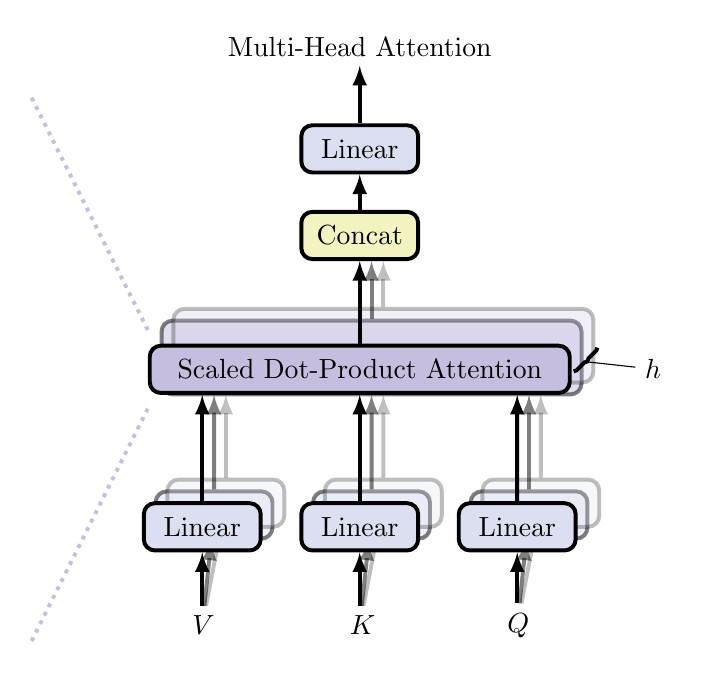
\begin{tikzpicture}[
    >=latex,
]

\definecolor{attention_func_color}{RGB}{197,190,223}
\definecolor{emb_color}{RGB}{252,224,225}
\definecolor{add_norm_color}{RGB}{242,243,193}
\definecolor{linear_color}{RGB}{220,223,240}

\tikzstyle{sqr} = [rectangle, rounded corners, minimum width=1cm, text width=1.25cm, minimum height=.6cm,text centered, draw=black, line width=.5mm]

\node (l1) [sqr, fill=linear_color] {Linear};
\node (V) [text width=.25cm, below of=l1, yshift=-.25cm] {$V$};
\begin{scope}[on  background layer]
\node (l11) [sqr, fill=linear_color, xshift=.15cm, yshift=.15cm, opacity=.5] {};
\draw[->, line width=.5mm, opacity=.5] (V) -- (l11);
\node (l12) [sqr, fill=linear_color, xshift=.3cm, yshift=.3cm, opacity=.25] {};
\draw[->, line width=.5mm, opacity=.25] (V) -- (l12);
\end{scope}

\node (l2) [sqr, fill=linear_color, right of=l1, xshift=1cm] {Linear};
\node (K) [text width=.25cm, below of=l2, yshift=-.25cm] {$K$};
\begin{scope}[on  background layer]
\node (l21) [sqr, fill=linear_color, right of=l1, xshift=1.15cm, yshift=.15cm, opacity=.5] {};
\draw[->, line width=.5mm, opacity=.5] (K) -- (l21);
\node (l22) [sqr, fill=linear_color, right of=l1, xshift=1.3cm, yshift=.3cm, opacity=.25] {};
\draw[->, line width=.5mm, opacity=.25] (K) -- (l22);
\end{scope}

\node (l3) [sqr, fill=linear_color, right of=l2, xshift=1cm] {Linear};
\node (Q) [text width=.25cm, below of=l3, yshift=-.25cm] {$Q$};
\begin{scope}[on  background layer]
\node (l31) [sqr, fill=linear_color, right of=l2, xshift=1.15cm, yshift=.15cm, opacity=.5] {};
\draw[->, line width=.5mm, opacity=.5] (Q) -- (l31);
\node (l32) [sqr, fill=linear_color, right of=l2, xshift=1.3cm, yshift=.3cm, opacity=.25] {};
\draw[->, line width=.5mm, opacity=.25] (Q) -- (l32);
\end{scope}

\node (attn) [sqr, fill=attention_func_color, above of=l2, xshift=0cm, text width=5.1cm, yshift=1cm] {Scaled Dot-Product Attention};
\begin{scope}[on  background layer]
    \node (attn1) [sqr, fill=attention_func_color, above of=l2, xshift=.15cm, text width=5.1cm, text height=2em, yshift=1.15cm, opacity=.5] {};
\node (attn2) [sqr, fill=attention_func_color, above of=l2, xshift=.3cm, text width=5.1cm, text height=2em, yshift=1.3cm, opacity=.25] {};
\end{scope}

\node (add1) [sqr, fill=add_norm_color, above of=attn, yshift=.7cm] {Concat};

\node (l4) [sqr, fill=linear_color, above of=add1, yshift=.1cm] {Linear};

\node (multih) [above of=l4, yshift=.3cm] {Multi-Head Attention};

\draw[->, line width=.5mm] (l1) -- ($(attn.south) + (-2cm, 0)$);
\draw[->, line width=.5mm, opacity=.5] (l11) -- ($(attn.south) + (-1.85cm, 0)$);
\draw[->, line width=.5mm, opacity=.25] (l12) -- ($(attn.south) + (-1.7cm, 0)$);

\draw[->, line width=.5mm] (l2) -- ($(attn.south) + (0, 0)$);
\draw[->, line width=.5mm, opacity=.5] (l21) -- ($(attn.south) + (.15cm, 0)$);
\draw[->, line width=.5mm, opacity=.25] (l22) -- ($(attn.south) + (.3cm, 0)$);

\draw[->, line width=.5mm] (l3) -- ($(attn.south) + (2cm, 0)$);
\draw[->, line width=.5mm, opacity=.5] (l31) -- ($(attn.south) + (2.15cm, 0)$);
\draw[->, line width=.5mm, opacity=.25] (l32) -- ($(attn.south) + (2.3cm, 0)$);

\draw[->, line width=.5mm] (attn.north) -- ($(add1.south) + (0, 0)$);
\draw[->, line width=.5mm, opacity=.5] (attn1.north) -- ($(add1.south) + (.15cm, 0)$);
\draw[->, line width=.5mm, opacity=.25] (attn2.north) -- ($(add1.south) + (.3cm, 0)$);

\draw[->, line width=.5mm] (add1) -- (l4);

\draw[->, line width=.5mm] (V) -- (l1);
\draw[->, line width=.5mm] (K) -- (l2);
\draw[->, line width=.5mm] (Q) -- (l3);

\draw[->, line width=.5mm] (l4.north) -- (multih.south);

\draw [decorate,decoration={brace,amplitude=1pt,mirror,raise=1pt},yshift=0pt, line width=.5mm] (attn.east) -- (attn2.east);
\node (h) [text width=.25cm, right of=attn, yshift=0, xshift=2.75cm] {$h$};
\draw [-] ($(attn.east) + (.15cm, .1cm)$) -- (h);

\draw[-, attention_func_color, line width=.5mm, dotted] ($ (attn.west) + (0, 0.5) $) -- ($(attn.west) + (-1.5, +3.5)$);
\draw[-, attention_func_color, line width=.5mm, dotted] ($ (attn.west) + (0, -0.5) $) -- ($(attn.west) + (-1.5, -3.5)$);

\end{tikzpicture}
